%  +---------------------------------+
%  | LaTeX template file for AES LAC |
%  +---------------------------------+
% This file is a modification of the template used for the
% AES Brazil.
% To be used with "aeslac.cls" version 1.0

%%
%% NOTE: This text file uses UNIX line feed conventions. When (human)
%% reading this file on other platforms, you may have to use a text
%% editor that can handle lines terminated by the UNIX line feed
%% character (0x0A).
%%

%%%%%%%%%%%%%%%%%%%%%%%%%%%%%%%%%%%%%%%%%%%%%%%%%%%%%%%%%%%
%
%  CARGADO DE LA CLASE
%
% La clase "aeslac.cls" carga automáticamente los siguientes paquetes:
%    hyperref, graphicx, color, times, y helvet.
% El paquete "graphicx.sty" es necesario para incluir imágenes,
% gráficos, etc. El uso de pdflatex requiere que el formato de las
% imágenes sea PDF, PNG, o JPG (no EPS).

% Para generar el documento en formato DVI, eliminar la opción 'pdfout'
% y ejecutar
% > latex template
% > bibtex template
% > latex template
%
% Para generar el documento en formato PDF ejecutar:
% > pdflatex template
% > bibtex template
% > pdflatex template

% Eliminar la opción "pdfout" si no se está usando 'pdflatex'.
% La opción "ams" carga los paquetes "amsmath", "amssymb" and "amsthm".
\documentclass
  [ams,pdfout]% opciones de la clase
	{aeslac}

%%%%%%%%%%%%%%%%%%%%%%%%%%%%%%%%%%%%%%%%%%%%%%%%%%%%%%%%%%%
%
% CARGADO DE PAQUETES
%
% Usar \RequirePackage en lugar de \usepackage
% Esto evita conflictos entre paquetes.

% Usar formato 8-bit UCS/Unicode Transformation Format
\RequirePackage[utf8]{inputenc}

% Para escribir el documento en español es necesario usar la opción
% "spanish" de "babel"
\RequirePackage[spanish]{babel}

% Usar caracteres extendidos
% Solo es necesario para escribir en portugués
\RequirePackage{textcomp}

\begin{document}
% La página del título es construida en el ambiente "TitlePage".
% En ese ambiente se genera el título, los autores y
% sus respectivas afiliaciones y el resumen, en ese orden.
\begin{TitlePage}
	% El titulo es producido con el comando \Title.
	\Title{Alineación Audio-Partitura para la flauta traversa}
	% \RunningTitle y \RunningAuthors son impresos en el
	% encabezado de cada página.
	\RunningTitle{Alineación Audio-Partitura para la flauta traversa} % titulo corto
	% 2 o mas autores:
	% ("Autor1 y Autor2" para 2 autores.)
	% ("Autor1 et al." para 3 o mas autores.)
	\RunningAuthors{Juan P. Braga Brum et al.}
% Especificar autor y afiliación (con \Author y \Affil) para cada
% autor (en ese orden).
% Primer autor
	\Author
		[juanbragabrum@gmail.com]% email
		{Juan P. Braga Brum} % Nombre del autor (impreso en la página del titulo)
		\Affil
			[A]% clave (argumento opcional)
			{%
				Universidad de la República (UdelaR),
				Facultad de Ingeniería (FIng),
				Instituto de Ingeniería Eléctrica (IIE)\\
				Montevideo, 11300, Uruguay
			}
	\Author
		[wagner@smt.ufrj.br]
		{L. W. P. Biscainho}
		\Affil
			[B]% clave (argumento opcional)
			{%
				Universidade Federal do Rio de Janeiro (UFRJ), 
				Escola Politécnica (Poli),
				Departamento de Engenharia Eletrônica e de Computação (DEL)\\
				Rio de Janeiro, RJ, 21941-972, Brasil
}
	\Author
		[obudon@vera.com.uy]
		{Osvaldo Budón}
		\Affil
			[C]% clave (argumento opcional)
			{%
				Universidad de la República (UdelaR),
				Escuela Universitaria de Música (EUMus),
				Instituo de Ingeniería Eléctrica\\
				Montevideo, 11200, Uruguay
}	
	
	
	\Author
		[pcancela@fing.edu.uy]
		{Pablo Cancela}
		\Affilref[A]
	
	\Abstract{%
		Un sistema de alineación entre audio y partitura para señales de flauta traversa es presentado. 
		Para eso, un abordaje desde el material sonoro generado de la flauta traversa es realizado. 
		La comparación de desempeño de varias estrategias en la base de datos de flauta tradicional es realizada.
		La base de datos queda disponible para futuros trabajos en el área.
		 
		%
	}%
\end{TitlePage}
%
% Los títulos de las secciones se escriben usando mayúsculas
\section{Introducción}

Música Electroacústica

Alineación Audio-Partitura

%
\subsection{Flauta traversa}

 


\subsection{Alcance y desarrollo de la publicacion}
%
\section{Alineación Audio-Partitura}
Historia

Solución

Dynamic Time Warping

\subsection{Estado del arte}
Carabias

\section{Metodología}
Enventanado

Extracción de contenido musical
	B3aB8 CQT
	Normalización
	12 bins Chroma

Codificación de la partitura
	Silencio
	Armónicos

Síntesis

Distancia Coseno


\section{Experimentos}

\subsection{Base de datos de flauta tradicional}


Características

Kaggle

\subsection{Resultados}
Comparación

Por Obra

\subsection{Técnicas extendidas}


\begin{table}[!ht]
\caption{Unidades SI y otras}
\label{tab:units}
\vspace*{10pt}
\centering
\small
\begin{tabular}{ll}
\textit{Nombre de la Unidad}	&	\textit{Símbolo de la Unidad}\\ \hline
ampere             		&	A\\
bit o bits        		&	como se escribe\\
bytes              		&	como se escribe\\
decibel           		&	dB\\
grado (geométrico)     	&	$^\textrm{o}$\\
farad             		&	F\\
gauss             		&	Gs\\
gramo             		&	g\\
henry              		&	H\\
hertz             		&	Hz\\
hora              		&	h\\
pulgada             		&	in\\
joule              		&	J\\
kelvin             		&	K\\
kilohertz          		&	kHz\\
kilohm                		&	k$\Omega$\\
litro             		&	l, L\\
megahertz         		&	MHz\\
metro              		&	m\\
microfarad         		&	$\mu$F\\
micrometro         		&	$\mu$m\\
microsegundo        		&	$\mu$s\\
milliampere        		&	mA\\
millihenry         		&	mH\\
millimetro         		&	mm\\
millivolt          		&	mV\\
minuto (tiempo)        		&	min\\
minuto (geométrico)     	&      	'\\
nanosegundo         		&	ns\\
oersted           		&	Oe\\
ohm                		&	$\Omega$\\
pascal             		&	Pa\\
picofarad          		&	pF\\
segundo (tiempo)      		&	s\\
segundo (geométrico)    	&	"\\
siemens            		&	S\\
tesla              		&	T\\
volt               		&	V\\
watt               		&	W\\
weber              		&	Wb\\
\end{tabular}
\end{table}
%
\section{DERECHOS DE AUTOR (COPYRIGHT)}

El texto entre líneas contenido en la parte superior de la primera página del artículo del congreso de la AES Latinoamérica, es propiedad de la \emph{Audio Engineering Society} y no puede ser reproducido sin permiso. Los derechos sobre el contenido de un artículo de congreso de la AES Latinoamérica pertenecen al autor o autores. Sin embargo, al entregar un artículo para presentar en un congreso de la AES, el autor estará aceptando que la \emph{AES Journal} tendrá la preferencia para su publicación. En el caso en que el artículo sea aceptado para ser publicado en la \emph{AES Journal} u otra ``\emph{Special Issue}'' de la \emph{AES}, la transferencia de los derechos será solicitada a los autores.
%


\begin{figure}[h!]
  \centering
	\ifpdfout
	    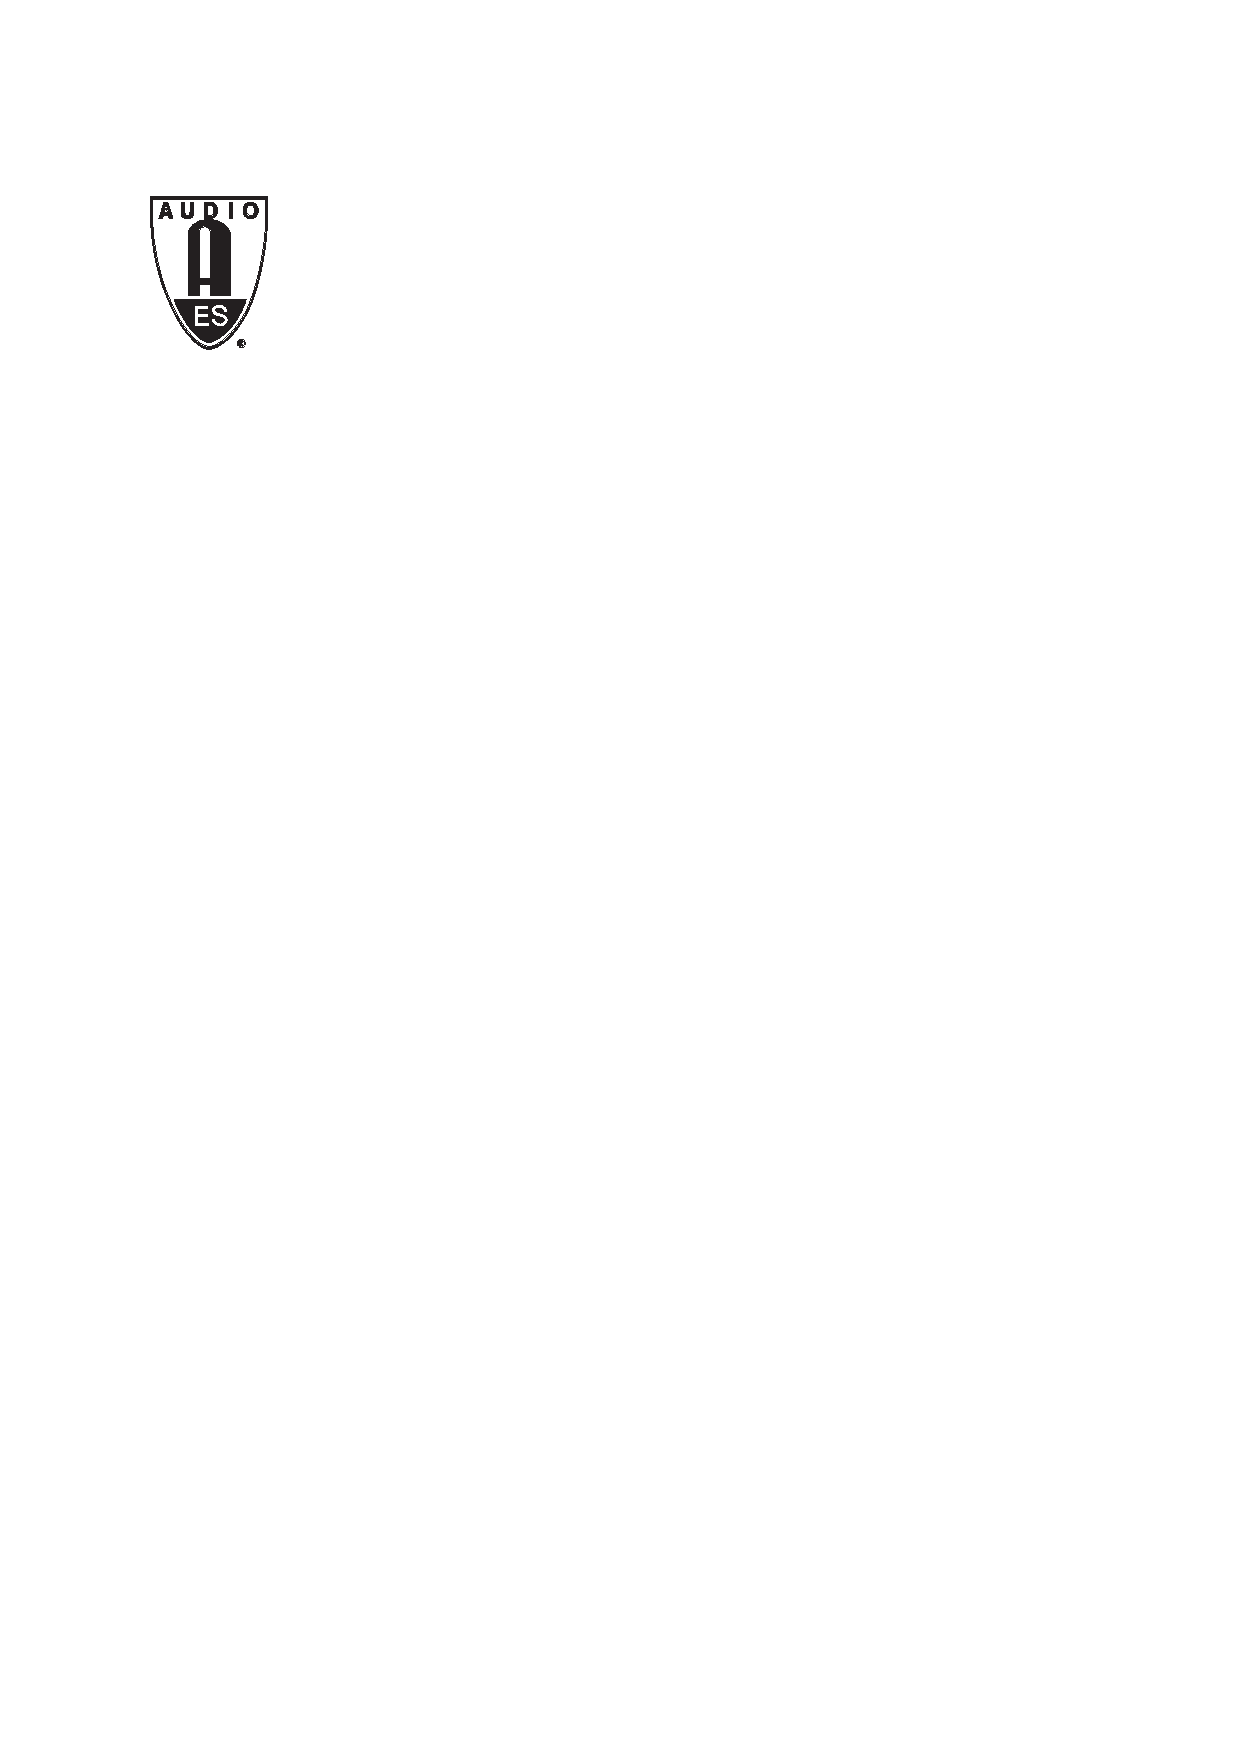
\includegraphics[width=3.4cm]{aeslogo.pdf}% (pdflatex)
	\else
	    
\includegraphics[width=3.4cm]{aeslogo.eps}% (latex)
	\fi
  \caption{Logotipo de la AES}
  \label{fig:logo}
\end{figure}

Las fotografías y las imágenes deben guardarse en baja resolución (de 72 a 300 dpi), manteniendo buena calidad y legibilidad.
%

\section{ECUACIONES}

Las ecuaciones son numeradas secuencialmente, entre paréntesis y en su propia línea. Se citan en el texto de la forma siguiente: ``Ecuación~(\ref{eq:1})''.

Para facilitar la composición de las fórmulas, utilice la opción de clase de documento \verb|ams|. Esta opción carga los paquetes \verb|amsmath|, \verb|amssymb| y \verb|amsthm|. Para incluir las ecuaciones en una línea separada del texto puede emplearse el ambiente \verb|equation|, como se muestra en el siguiente ejemplo:
\begin{equation}
\label{eq:1}
  \left\{\,
    x\biggm|\int_{0}^x t^{2}\,dt\leq5
  \,\right\}.
\end{equation}

Las ecuaciones que superan el ancho de una columna pueden ajustarse en dos líneas; eso se puede hacer con el paquete \verb|breqn|, usado para separar una ecuación en dos o mas líneas.

%%%%%%%%%%%%%%%%%%%%%%%%%%%%%%%%%%%%%%%%%%%%%%%%%%%%%%%%%%%
%
% EJEMPLO DE BIBLIOGRAFÍA
%
% para generar la bibliografía ejecutar "bibtex template"
\bibliographystyle{aes} % estilo aes.bst
\bibliography{bib} % archivo de bibliografía en formato bibtex
%
\end{document} 